% =========================================================================
% BÀI 15: VỊ TRÍ, ĐỊNH HƯỚNG TRONG KHÔNG GIAN (CHỦ ĐỀ 4 - TOÁN LỚP 1)
% TOÀN BỘ CÂU HỎI ĐƯỢC VẼ HÌNH MINH HỌA TRỰC QUAN 100% BẰNG TIKZ
% =========================================================================

% --- CÁC HÀM VẼ ĐỒ VẬT VÀ KHÔNG GIAN CHO BÀI 15 ---
\providecommand{\VeBanHoc}[2]{% #1=x, #2=y
  \begin{scope}[shift={(#1,#2)}]
    % Mặt bàn
    \draw[fill=brown!40, draw=brown!85!black, line width=1.3pt] (-2.2,0) -- (1.8,0) -- (2.3,0.6) -- (-1.7,0.6) -- cycle;
    % Yếm bàn
    \draw[fill=brown!60!black, draw=brown!85!black, line width=1pt] (-2.2,-0.15) rectangle (1.8,0);
    % 4 chân bàn
    \draw[fill=brown!70!black, draw=brown!90!black, line width=1pt] (-2.1,-1.2) rectangle (-1.9,-0.15);
    \draw[fill=brown!70!black, draw=brown!90!black, line width=1pt] (1.5,-1.2) rectangle (1.7,-0.15);
    \draw[fill=brown!50!black, draw=brown!80!black, line width=0.8pt] (-1.6,-0.8) rectangle (-1.45,0);
    \draw[fill=brown!50!black, draw=brown!80!black, line width=0.8pt] (1.9,-0.8) rectangle (2.05,0.45);
  \end{scope}
}

\providecommand{\VeBanNho}[3][blue!70]{% #1=màu áo, #2=x, #3=y
  \begin{scope}[shift={(#2,#3)}, scale=0.55]
    \fill[orange!22] (0, 0.55) circle (0.22cm);
    \fill[brown!80!black] (-0.22,0.6) arc (180:0:0.22cm) -- cycle;
    \fill[black] (-0.08,0.56) circle (0.025cm);
    \fill[black] (0.08,0.56) circle (0.025cm);
    \draw[line width=0.6pt, red!70!black] (-0.06,0.48) arc (-150:-30:0.07cm);
    \fill[#1] (-0.16,0.1) rectangle (0.16,0.38);
    \draw[line width=1.3pt, blue!90!black] (-0.08,0.1) -- (-0.08,-0.12);
    \draw[line width=1.3pt, blue!90!black] (0.08,0.1) -- (0.08,-0.12);
  \end{scope}
}

\providecommand{\VeChuMeo}[2]{% #1=x, #2=y
  \begin{scope}[shift={(#1,#2)}, scale=0.5]
    \fill[orange!85!black] (0,0) ellipse (0.35cm and 0.22cm);
    \fill[orange!85!black] (0.28,0.15) circle (0.18cm);
    \fill[orange!95!black] (0.2,0.28) -- (0.25,0.42) -- (0.32,0.3) -- cycle;
    \fill[orange!95!black] (0.3,0.28) -- (0.38,0.42) -- (0.42,0.28) -- cycle;
    \fill[black] (0.32,0.18) circle (0.03cm);
    \draw[line width=1pt, orange!90!black] (-0.3,0) to[out=150,in=-30] (-0.55,0.25);
  \end{scope}
}

\providecommand{\VeQuaBong}[2]{% #1=x, #2=y
  \begin{scope}[shift={(#1,#2)}]
    \shade[ball color=red!85!white] (0,0) circle (0.28cm);
  \end{scope}
}

\providecommand{\VeCayXanh}[2]{% #1=x, #2=y
  \begin{scope}[shift={(#1,#2)}, scale=0.65]
    \fill[brown!75!black] (-0.15,-1.2) rectangle (0.15,0);
    \fill[green!65!black] (0,0.6) circle (0.55cm);
    \fill[green!75!black] (-0.45,0.1) circle (0.45cm);
    \fill[green!75!black] (0.45,0.1) circle (0.45cm);
    \fill[green!70!black] (0,0) circle (0.5cm);
  \end{scope}
}

% =========================================================================
% PHẦN 1: TRẮC NGHIỆM LỰA CHỌN (12 CÂU)
% =========================================================================
\textbf{Phần 1. Trắc nghiệm lựa chọn}
\setcounterpageref{ex}{0}

% --- CÂU 1 ---
\begin{ex} %[1H4N15]
Bé xòe hai bàn tay như hình vẽ. Bạn nhỏ đang cầm chiếc bút chì ở phía tay nào?
\begin{center}
\begin{tikzpicture}[scale=0.85, baseline=(current bounding box.center)]
  % Tay trái trống
  \draw[fill=orange!25, draw=orange!80!black, line width=1.1pt, rounded corners=3pt] (-2.2,-0.5) rectangle (-1.2,0.5);
  \node[font=\footnotesize\bfseries\color{blue!80!black}] at (-1.7,-0.75) {Tay trái (trống)};
  
  % Mặt bạn cười ở giữa
  \fill[orange!22] (0,0.2) circle (0.45cm);
  \fill[black] (-0.15,0.28) circle (0.04cm);
  \fill[black] (0.15,0.28) circle (0.04cm);
  \draw[line width=1pt, red!75!black] (-0.12,0.08) arc (-150:-30:0.14cm);
  
  % Tay phải cầm bút
  \draw[fill=orange!25, draw=orange!80!black, line width=1.1pt, rounded corners=3pt] (1.2,-0.5) rectangle (2.2,0.5);
  % Bút chì
  \draw[fill=yellow!80!orange, draw=orange!90!black, line width=0.8pt] (1.6,-0.3) rectangle (1.8,0.7);
  \fill[brown!80!black] (1.6,0.7) -- (1.7,0.95) -- (1.8,0.7) -- cycle;
  \fill[black] (1.68,0.9) -- (1.7,0.95) -- (1.72,0.9) -- cycle;
  \node[font=\footnotesize\bfseries\color{red!85!black}] at (1.7,-0.75) {Tay phải (cầm bút)};
\end{tikzpicture}
\end{center}
\choice
{Tay trái}
{Cả hai tay}
{Bàn chân}
{\True Tay phải}
\loigiai{
Chiếc bút chì đang được cầm ở phía \textbf{tay phải}.\\
\textbf{Đáp án của câu hỏi là D}
}
\end{ex}

% --- CÂU 2 ---
\begin{ex} %[1H4N15]
Quan sát 3 bạn nhỏ xếp hàng: bạn đội mũ vàng, bạn áo xanh và bạn đeo ba lô. Bạn đội mũ vàng đang đứng ở vị trí nào so với bạn áo xanh?
\begin{center}
\begin{tikzpicture}[scale=0.85, baseline=(current bounding box.center)]
  % Mũi tên hướng đi về phía trước
  \draw[->, >=stealth, line width=1.4pt, orange!90!black] (-3.8,0) -- (-4.6,0);
  \node[above=2pt, font=\scriptsize\bfseries\color{orange!90!black}] at (-4.2,0) {Phía trước};
  
  % Bạn 1 (đội mũ vàng)
  \VeBanNho[yellow!80!orange]{-3.0}{0}
  \fill[yellow!90!black] (-3.15,0.3) rectangle (-2.85,0.45);
  \node[below=4pt, font=\scriptsize\bfseries\color{orange!90!black}] at (-3.0,-0.1) {Bạn mũ vàng};
  
  % Bạn 2 (áo xanh)
  \VeBanNho[blue!75]{-1.0}{0}
  \node[below=4pt, font=\scriptsize\bfseries\color{blue!85!black}] at (-1.0,-0.1) {Bạn áo xanh};
  
  % Bạn 3 (đeo ba lô)
  \VeBanNho[red!75]{1.0}{0}
  \fill[brown!80!black] (1.1,0.05) rectangle (1.25,0.25);
  \node[below=4pt, font=\scriptsize\bfseries\color{red!85!black}] at (1.0,-0.1) {Bạn ba lô};
\end{tikzpicture}
\end{center}
\choice
{\True Ở trước}
{Ở sau}
{Bên trái}
{Bên phải}
\loigiai{
Bạn đội mũ vàng đang đứng \textbf{ở trước} bạn áo xanh.\\
\textbf{Đáp án của câu hỏi là A}
}
\end{ex}

% --- CÂU 3 ---
\begin{ex} %[1H4H15]
Quan sát hình chiếc bàn học: chú mèo lười đang nằm ở vị trí nào so với mặt bàn?
\begin{center}
\begin{tikzpicture}[scale=0.85, baseline=(current bounding box.center)]
  \VeBanHoc{0}{0}
  % Lọ hoa trên bàn
  \fill[cyan!40, draw=blue!85!black, line width=0.8pt] (0,0.15) rectangle (0.5,0.65);
  \node[font=\tiny\bfseries\color{blue!90!black}] at (0.25,0.4) {Lọ hoa};
  
  % Chú mèo dưới gầm bàn
  \VeChuMeo{-0.4}{-0.9}
  \node[below=3pt, font=\small\bfseries\color{orange!90!black}] at (-0.2,-1.0) {Chú mèo lười};
\end{tikzpicture}
\end{center}
\choice
{Ở trên}
{\True Ở dưới (dưới gầm bàn)}
{Ở sau}
{Ở giữa}
\loigiai{
Chú mèo đang nằm \textbf{ở dưới} gầm bàn.\\
\textbf{Đáp án của câu hỏi là B}
}
\end{ex}

% --- CÂU 4 ---
\begin{ex} %[1H4H15]
Chiếc đèn học treo ở vị trí nào so với mặt bàn học?
\begin{center}
\begin{tikzpicture}[scale=0.85, baseline=(current bounding box.center)]
  \VeBanHoc{0}{0}
  % Đèn học ở trên
  \draw[line width=1.2pt, gray!80!black] (0,1.8) -- (0,1.1);
  \draw[fill=yellow!80!orange, draw=orange!90!black, line width=1.1pt] (-0.4,0.8) -- (0.4,0.8) -- (0.25,1.1) -- (-0.25,1.1) -- cycle;
  \node[right=5pt, font=\small\bfseries\color{orange!90!black}] at (0.4,0.95) {Đèn học};
\end{tikzpicture}
\end{center}
\choice
{Ở dưới}
{\True Ở trên}
{Ở sau}
{Bên trái}
\loigiai{
Chiếc đèn học ở vị trí \textbf{ở trên} so với mặt bàn.\\
\textbf{Đáp án của câu hỏi là B}
}
\end{ex}

\newpage
% --- CÂU 5 ---
\begin{ex} %[1H4H15]
Trong bức tranh dưới đây, bạn Hoa đang đứng ở vị trí nào so với bạn Nam và bạn Mai?
\begin{center}
\begin{tikzpicture}[scale=0.85, baseline=(current bounding box.center)]
  \VeBanNho[blue!75]{-2.2}{0}
  \node[below=3pt, font=\small\bfseries\color{blue!85!black}] at (-2.2,-0.1) {Bạn Nam};
  
  \VeBanNho[magenta!75]{0}{0}
  \node[below=3pt, font=\small\bfseries\color{magenta!85!black}] at (0,-0.1) {Bạn Hoa};
  
  \VeBanNho[green!70!black]{2.2}{0}
  \node[below=3pt, font=\small\bfseries\color{green!70!black}] at (2.2,-0.1) {Bạn Mai};
\end{tikzpicture}
\end{center}
\choice
{Ở ngoài cùng bên trái}
{Ở trên}
{\True Ở giữa}
{Ở dưới}
\loigiai{
Bạn Hoa đứng \textbf{ở giữa} bạn Nam và bạn Mai.\\
\textbf{Đáp án của câu hỏi là C}
}
\end{ex}

% --- CÂU 6 ---
\begin{ex} %[1H4H15]
Khi đi bộ trên đường giao thông, em cần đi về phía bên nào theo quy định?
\begin{center}
\begin{tikzpicture}[scale=0.85, baseline=(current bounding box.center)]
  \draw[fill=gray!20, draw=gray!70!black, line width=1.2pt] (-3.2,-0.8) rectangle (3.2,0.8);
  \draw[dashed, line width=1.2pt, yellow!90!black] (-3.2,0) -- (3.2,0);
  
  \node[font=\small\bfseries\color{gray!80!black}] at (-1.6,0.35) {Phía bên trái};
  \node[font=\small\bfseries\color{blue!90!black}] at (1.6,-0.35) {Phía bên phải};
  \draw[->, >=stealth, line width=1.6pt, blue!90!black] (0.8,-0.35) -- (2.4,-0.35);
\end{tikzpicture}
\end{center}
\choice
{Bên trái}
{Đi giữa lòng đường}
{Đi tùy ý}
{\True Bên phải}
\loigiai{
Khi tham gia giao thông, em cần đi về phía \textbf{bên phải}.\\
\textbf{Đáp án của câu hỏi là D}
}
\end{ex}

% --- CÂU 7 ---
\begin{ex} %[1H4V15]
Quan sát hình vẽ: chú chim đang đậu trên cành cây, chú rùa đang bò trên mặt đất. Chú chim ở vị trí nào so với chú rùa?
\begin{center}
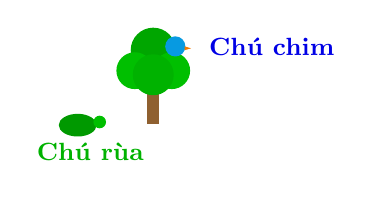
\begin{tikzpicture}[scale=0.8, baseline=(current bounding box.center)]
  \VeCayXanh{0}{0}
  % Chú chim trên cành
  \fill[cyan!85!blue] (0.35,0.45) circle (0.16cm);
  \fill[orange!95!black] (0.5,0.45) -- (0.6,0.42) -- (0.5,0.39) -- cycle;
  \node[right=3pt, font=\small\bfseries\color{blue!90!black}] at (0.6,0.45) {Chú chim};
  
  % Chú rùa dưới đất
  \fill[green!60!black] (-1.2,-0.8) ellipse (0.3cm and 0.18cm);
  \fill[green!75!black] (-0.85,-0.75) circle (0.1cm);
  \node[below=3pt, font=\small\bfseries\color{green!70!black}] at (-1.0,-0.8) {Chú rùa};
\end{tikzpicture}
\end{center}
\choice
{\True Ở trên}
{Ở dưới}
{Ở sau}
{Ở giữa}
\loigiai{
Chú chim ở vị trí \textbf{ở trên} so với chú rùa.\\
\textbf{Đáp án của câu hỏi là A}
}
\end{ex}

% --- CÂU 8 ---
\begin{ex} %[1H4V15]
Chiếc giá sách có 3 ngăn: ngăn trên đựng sách, ngăn giữa đựng gấu bông, ngăn dưới đựng quả bóng. Gấu bông nằm ở ngăn nào?
\begin{center}
\begin{tikzpicture}[scale=0.8, baseline=(current bounding box.center)]
  % Khung giá sách 3 tầng
  \draw[fill=brown!20, draw=brown!85!black, line width=1.3pt] (-1.8,-1.5) rectangle (1.8,1.5);
  \draw[line width=1.2pt, brown!85!black] (-1.8,-0.5) -- (1.8,-0.5);
  \draw[line width=1.2pt, brown!85!black] (-1.8,0.5) -- (1.8,0.5);
  
  \node[font=\small\bfseries\color{blue!85!black}] at (0,1.0) {Ngăn trên: Sách vở};
  \node[font=\small\bfseries\color{red!85!black}] at (0,0) {Ngăn giữa: Gấu bông};
  \node[font=\small\bfseries\color{green!70!black}] at (0,-1.0) {Ngăn dưới: Quả bóng};
\end{tikzpicture}
\end{center}
\choice
{Ngăn trên}
{Ngăn dưới}
{\True Ngăn giữa}
{Ngoài giá sách}
\loigiai{
Gấu bông nằm ở \textbf{ngăn giữa}.\\
\textbf{Đáp án của câu hỏi là C}
}
\end{ex}

\newpage
% --- CÂU 9 ---
\begin{ex} %[1H4V15]
Trên đường đi, chiếc xe ô tô màu đỏ chạy phía trước, chiếc xe máy chạy phía sau xe ô tô. Chiếc xe máy đang chạy ở vị trí nào?
\begin{center}
\begin{tikzpicture}[scale=0.8, baseline=(current bounding box.center)]
  % Mũi tên chiều chuyển động sang trái
  \draw[->, >=stealth, line width=1.4pt, orange!90!black] (-3.2,0.8) -- (-4.2,0.8);
  \node[above=2pt, font=\scriptsize\bfseries\color{orange!90!black}] at (-3.7,0.8) {Hướng chạy};
  
  % Xe ô tô (ở trước)
  \draw[fill=red!75!black, draw=red!90!black, line width=1.1pt, rounded corners=3pt] (-3.2,-0.3) rectangle (-1.2,0.4);
  \fill[black] (-2.8,-0.3) circle (0.15cm);
  \fill[black] (-1.6,-0.3) circle (0.15cm);
  \node[below=4pt, font=\small\bfseries\color{red!85!black}] at (-2.2,-0.4) {Xe ô tô (ở trước)};
  
  % Xe máy (ở sau)
  \draw[fill=cyan!60!blue, draw=blue!90!black, line width=1.1pt] (1.2,-0.2) rectangle (2.4,0.3);
  \fill[black] (1.4,-0.25) circle (0.14cm);
  \fill[black] (2.2,-0.25) circle (0.14cm);
  \node[below=4pt, font=\small\bfseries\color{blue!85!black}] at (1.8,-0.4) {Xe máy (ở sau)};
\end{tikzpicture}
\end{center}
\choice
{\True Ở sau}
{Ở trước}
{Ở trên}
{Ở dưới}
\loigiai{
Chiếc xe máy đang chạy \textbf{ở sau} chiếc xe ô tô.\\
\textbf{Đáp án của câu hỏi là A}
}
\end{ex}

% --- CÂU 10 ---
\begin{ex} %[1H4V15]
Quan sát hai đĩa quả: đĩa bên trái đựng quả táo, đĩa bên phải đựng quả cam. Quả cam nằm ở đĩa phía bên nào?
\begin{center}
\begin{tikzpicture}[scale=0.8, baseline=(current bounding box.center)]
  % Đĩa trái (táo)
  \draw[fill=orange!15, draw=orange!80!black, line width=1.2pt] (-2.2,-0.2) ellipse (1.2cm and 0.4cm);
  \fill[red!85!black] (-2.2,0.1) circle (0.25cm);
  \node[below=4pt, font=\small\bfseries\color{red!85!black}] at (-2.2,-0.35) {Đĩa bên trái (Táo)};
  
  % Đĩa phải (cam)
  \draw[fill=orange!15, draw=orange!80!black, line width=1.2pt] (2.2,-0.2) ellipse (1.2cm and 0.4cm);
  \fill[orange!90!black] (2.2,0.1) circle (0.25cm);
  \node[below=4pt, font=\small\bfseries\color{orange!90!black}] at (2.2,-0.35) {Đĩa bên phải (Cam)};
\end{tikzpicture}
\end{center}
\choice
{Bên trái}
{Ở trên}
{\True Bên phải}
{Ở dưới}
\loigiai{
Quả cam nằm ở đĩa phía \textbf{bên phải}.\\
\textbf{Đáp án của câu hỏi là C}
}
\end{ex}

% --- CÂU 11 ---
\begin{ex} %[1H4V15]
Ngôi nhà ngói đỏ nằm ở vị trí nào so với hai cây xanh?
\begin{center}
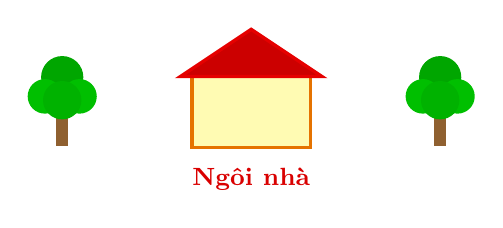
\begin{tikzpicture}[scale=0.75, baseline=(current bounding box.center)]
  \VeCayXanh{-3.2}{0}
  
  % Ngôi nhà ở giữa
  \draw[fill=yellow!30, draw=orange!90!black, line width=1.2pt] (-1.0,-0.8) rectangle (1.0,0.4);
  \draw[fill=red!80!black, draw=red!90!black, line width=1.2pt] (-1.2,0.4) -- (0,1.2) -- (1.2,0.4) -- cycle;
  \node[below=4pt, font=\small\bfseries\color{red!85!black}] at (0,-0.8) {Ngôi nhà};
  
  \VeCayXanh{3.2}{0}
\end{tikzpicture}
\end{center}
\choice
{Bên trái}
{Bên phải}
{Ở trên}
{\True Ở giữa}
\loigiai{
Ngôi nhà nằm \textbf{ở giữa} hai cây xanh.\\
\textbf{Đáp án của câu hỏi là D}
}
\end{ex}

% --- CÂU 12 ---
\begin{ex} %[1H4C15]
Bức tranh chụp gia đình: Bố đứng bên trái, Mẹ đứng bên phải, bạn nhỏ đứng ở giữa. Bạn nhỏ đứng ở vị trí nào?
\begin{center}
\begin{tikzpicture}[scale=0.8, baseline=(current bounding box.center)]
  \VeBanNho[blue!80]{-2.2}{0}
  \node[below=3pt, font=\small\bfseries\color{blue!85!black}] at (-2.2,-0.1) {Bố (bên trái)};
  
  \VeBanNho[yellow!85!orange]{0}{-0.2}
  \node[below=3pt, font=\small\bfseries\color{orange!90!black}] at (0,-0.3) {Bé};
  
  \VeBanNho[pink!80!red]{2.2}{0}
  \node[below=3pt, font=\small\bfseries\color{red!85!black}] at (2.2,-0.1) {Mẹ (bên phải)};
\end{tikzpicture}
\end{center}
\choice
{Bên trái}
{\True Ở giữa}
{Bên phải}
{Ở đằng sau}
\loigiai{
Bạn nhỏ đứng \textbf{ở giữa} bố và mẹ.\\
\textbf{Đáp án của câu hỏi là B}
}
\end{ex}

\newpage
% =========================================================================
% PHẦN 2: TRẮC NGHIỆM ĐÚNG SAI (2 CÂU)
% =========================================================================
\textbf{Phần 2. Trắc nghiệm đúng sai}
\setcounterpageref{ex}{0}

% --- CÂU 13 ---
\begin{ex} %[1H4H15]
Quan sát bức tranh chiếc bàn học dưới đây:
\begin{center}
\begin{tikzpicture}[scale=0.85, baseline=(current bounding box.center)]
  \VeBanHoc{0}{0}
  % Quyển vở trên bàn
  \draw[fill=cyan!30, draw=blue!85!black, line width=0.8pt] (-0.8,0.1) rectangle (-0.2,0.45);
  \node[font=\tiny\bfseries\color{blue!85!black}] at (-0.5,0.28) {Vở};
  
  % Hộp bút bên phải mặt bàn
  \draw[fill=yellow!40, draw=orange!90!black, line width=0.8pt] (0.4,0.1) rectangle (1.1,0.35);
  \node[font=\tiny\bfseries\color{orange!90!black}] at (0.75,0.22) {Hộp bút};
  
  % Quả bóng dưới gầm bàn
  \VeQuaBong{0}{-0.8}
  \node[font=\tiny\bfseries\color{red!85!black}] at (0,-1.15) {Bóng};
\end{tikzpicture}
\end{center}
Xét tính đúng sai của các câu sau:
\choiceTF
{\True Quyển vở ở trên mặt bàn.}
{\True Quả bóng ở dưới gầm bàn.}
{Hộp bút nằm ở phía bên trái của quyển vở.}
{\True Hộp bút nằm ở phía bên phải của quyển vở.}
\loigiai{
\begin{itemize}
    \item a) \textbf{Đúng}: Quyển vở nằm trên mặt bàn.
    \item b) \textbf{Đúng}: Quả bóng ở dưới gầm bàn.
    \item c) \textbf{Sai}: Hộp bút nằm ở phía bên phải quyển vở, không phải bên trái.
    \item d) \textbf{Đúng}: Hộp bút ở phía bên phải.
\end{itemize}
}
\end{ex}

% --- CÂU 14 ---
\begin{ex} %[1H4V15]
Đoàn tàu hỏa gồm đầu tàu và 3 toa xe đang chạy về phía bên trái:
\begin{center}
\begin{tikzpicture}[scale=0.75, baseline=(current bounding box.center)]
  % Hướng chạy sang trái
  \draw[->, >=stealth, line width=1.4pt, orange!90!black] (-4.5,0.6) -- (-5.3,0.6);
  
  % Đầu tàu
  \draw[fill=red!75!black, draw=red!90!black, line width=1pt] (-4.2,-0.4) rectangle (-2.8,0.4);
  \node[font=\tiny\bfseries\color{white}] at (-3.5,0) {Đầu tàu};
  \fill[black] (-3.9,-0.45) circle (0.12cm);
  \fill[black] (-3.1,-0.45) circle (0.12cm);
  
  % Nối toa
  \draw[line width=2pt, black] (-2.8,-0.1) -- (-2.4,-0.1);
  
  % Toa 1
  \draw[fill=yellow!60, draw=orange!90!black, line width=1pt] (-2.4,-0.4) rectangle (-1.0,0.4);
  \node[font=\small\bfseries\color{orange!90!black}] at (-1.7,0) {Toa 1};
  \fill[black] (-2.1,-0.45) circle (0.12cm);
  \fill[black] (-1.3,-0.45) circle (0.12cm);
  
  % Nối toa
  \draw[line width=2pt, black] (-1.0,-0.1) -- (-0.6,-0.1);
  
  % Toa 2
  \draw[fill=green!40, draw=green!70!black, line width=1pt] (-0.6,-0.4) rectangle (0.8,0.4);
  \node[font=\small\bfseries\color{green!70!black}] at (0.1,0) {Toa 2};
  \fill[black] (-0.3,-0.45) circle (0.12cm);
  \fill[black] (0.5,-0.45) circle (0.12cm);
  
  % Nối toa
  \draw[line width=2pt, black] (0.8,-0.1) -- (1.2,-0.1);
  
  % Toa 3
  \draw[fill=cyan!40, draw=blue!85!black, line width=1pt] (1.2,-0.4) rectangle (2.6,0.4);
  \node[font=\small\bfseries\color{blue!90!black}] at (1.9,0) {Toa 3};
  \fill[black] (1.5,-0.45) circle (0.12cm);
  \fill[black] (2.3,-0.45) circle (0.12cm);
\end{tikzpicture}
\end{center}
Xét tính đúng sai của các câu sau:
\choiceTF
{\True Đầu tàu hỏa chạy ở phía trước.}
{\True Toa 3 chạy ở sau cùng.}
{Toa 2 chạy ở phía trước Toa 1.}
{\True Toa 2 ở giữa Toa 1 và Toa 3.}
\loigiai{
\begin{itemize}
    \item a) \textbf{Đúng}: Đầu tàu ở trước nhất.
    \item b) \textbf{Đúng}: Toa 3 ở sau cùng.
    \item c) \textbf{Sai}: Toa 2 ở sau Toa 1.
    \item d) \textbf{Đúng}: Toa 2 nằm ở giữa Toa 1 và Toa 3.
\end{itemize}
}
\end{ex}

% =========================================================================
% PHẦN 3: TRẢ LỜI NGẮN (6 CÂU)
% =========================================================================
\textbf{Phần 3. Trả lời ngắn (Quan sát hình vẽ và điền số thích hợp)}
\setcounterpageref{ex}{0}

% --- CÂU 15 ---
\begin{ex} %[1H4H15]
Có bao nhiêu quyển sách nằm ở \textbf{TRÊN} mặt bàn?
\begin{center}
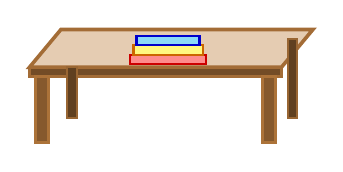
\begin{tikzpicture}[scale=0.8, baseline=(current bounding box.center)]
  \VeBanHoc{0}{0}
  % 3 quyển sách chồng lên nhau
  \draw[fill=red!45, draw=red!80!black, line width=0.8pt] (-0.6,0.05) rectangle (0.6,0.2);
  \draw[fill=yellow!50, draw=orange!80!black, line width=0.8pt] (-0.55,0.2) rectangle (0.55,0.35);
  \draw[fill=cyan!45, draw=blue!80!black, line width=0.8pt] (-0.5,0.35) rectangle (0.5,0.5);
\end{tikzpicture}
\end{center}
\shortans{3}
\loigiai{
\textbf{Đáp số:} $3$\\
Có $3$ quyển sách ở trên mặt bàn.
}
\end{ex}

% --- CÂU 16 ---
\begin{ex} %[1H4H15]
Có bao nhiêu chú cá bơi ở \textbf{DƯỚI} làn nước?
\begin{center}
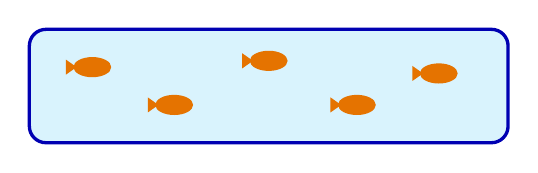
\begin{tikzpicture}[scale=0.8, baseline=(current bounding box.center)]
  \draw[fill=cyan!15, draw=blue!70!black, line width=1.2pt, rounded corners=6pt] (-3.8,-0.9) rectangle (3.8,0.9);
  \foreach \x/\y in {-2.8/0.3, -1.5/-0.3, 0/0.4, 1.4/-0.3, 2.7/0.2} {
    \fill[orange!90!black] (\x,\y) ellipse (0.3cm and 0.16cm);
    \fill[orange!90!black] (\x-0.25,\y) -- (\x-0.42,\y+0.12) -- (\x-0.42,\y-0.12) -- cycle;
  }
\end{tikzpicture}
\end{center}
\shortans{5}
\loigiai{
\textbf{Đáp số:} $5$\\
Có $5$ chú cá bơi ở dưới nước.
}
\end{ex}

\newpage
% --- CÂU 17 ---
\begin{ex} %[1H4V15]
Có 4 bạn nhỏ xếp hàng đứng \textbf{ở trước} bạn Minh. Hỏi có bao nhiêu bạn đứng trước bạn Minh?
\begin{center}
\begin{tikzpicture}[scale=0.75, baseline=(current bounding box.center)]
  \draw[->, >=stealth, line width=1.3pt, orange!90!black] (-4.5,0.4) -- (-5.2,0.4);
  \foreach \i in {0,1,2,3} {
    \VeBanNho[blue!75]{\i*1.2 - 4.0}{0}
  }
  \node[below=3pt, font=\small\bfseries\color{blue!90!black}] at (-2.2,-0.1) {4 bạn đứng trước};
  
  \VeBanNho[red!75]{1.2}{0}
  \node[below=3pt, font=\small\bfseries\color{red!85!black}] at (1.2,-0.1) {Bạn Minh};
\end{tikzpicture}
\end{center}
\shortans{4}
\loigiai{
\textbf{Đáp số:} $4$\\
Có $4$ bạn đứng trước bạn Minh.
}
\end{ex}

% --- CÂU 18 ---
\begin{ex} %[1H4V15]
Đĩa bên \textbf{TRÁI} có bao nhiêu quả táo đỏ?
\begin{center}
\begin{tikzpicture}[scale=0.8, baseline=(current bounding box.center)]
  % Đĩa trái (4 quả)
  \draw[fill=orange!15, draw=orange!80!black, line width=1.2pt] (-2.4,-0.2) ellipse (1.6cm and 0.45cm);
  \foreach \i in {0,1,2,3} {
    \fill[red!85!black] (\i*0.65 - 3.4, 0.05) circle (0.22cm);
  }
  \node[below=3pt, font=\small\bfseries\color{red!85!black}] at (-2.4,-0.35) {Đĩa bên trái};
  
  % Đĩa phải (2 quả)
  \draw[fill=orange!15, draw=orange!80!black, line width=1.2pt] (2.4,-0.2) ellipse (1.2cm and 0.4cm);
  \fill[green!75!black] (2.1,0.05) circle (0.22cm);
  \fill[green!75!black] (2.7,0.05) circle (0.22cm);
  \node[below=3pt, font=\small\bfseries\color{green!70!black}] at (2.4,-0.35) {Đĩa bên phải};
\end{tikzpicture}
\end{center}
\shortans{4}
\loigiai{
\textbf{Đáp số:} $4$\\
Đĩa bên trái có $4$ quả táo đỏ.
}
\end{ex}

% --- CÂU 19 ---
\begin{ex} %[1H4V15]
Đĩa bên \textbf{PHẢI} có bao nhiêu quả cam?
\begin{center}
\begin{tikzpicture}[scale=0.8, baseline=(current bounding box.center)]
  % Đĩa trái (3 quả)
  \draw[fill=orange!15, draw=orange!80!black, line width=1.2pt] (-2.4,-0.2) ellipse (1.3cm and 0.4cm);
  \foreach \i in {0,1,2} {
    \fill[red!85!black] (\i*0.6 - 3.0, 0.05) circle (0.22cm);
  }
  \node[below=3pt, font=\small\bfseries\color{red!85!black}] at (-2.4,-0.35) {Đĩa bên trái};
  
  % Đĩa phải (5 quả cam)
  \draw[fill=orange!15, draw=orange!80!black, line width=1.2pt] (2.4,-0.2) ellipse (1.6cm and 0.45cm);
  \foreach \i in {0,1,2,3,4} {
    \fill[orange!90!black] (\i*0.55 + 1.3, 0.05) circle (0.22cm);
  }
  \node[below=3pt, font=\small\bfseries\color{orange!90!black}] at (2.4,-0.35) {Đĩa bên phải};
\end{tikzpicture}
\end{center}
\shortans{5}
\loigiai{
\textbf{Đáp số:} $5$\\
Đĩa bên phải có $5$ quả cam.
}
\end{ex}

% --- CÂU 20 ---
\begin{ex} %[1H4C15]
Trên giá sách có tất cả 7 quyển truyện gồm ngăn trên và ngăn dưới. Biết ngăn trên có 4 quyển truyện, hỏi ngăn dưới có bao nhiêu quyển truyện?
\begin{center}
\begin{tikzpicture}[scale=0.8, baseline=(current bounding box.center)]
  \draw[fill=brown!15, draw=brown!85!black, line width=1.2pt] (-2.2,-1.1) rectangle (2.2,1.1);
  \draw[line width=1.2pt, brown!85!black] (-2.2,0) -- (2.2,0);
  \node[font=\small\bfseries\color{blue!85!black}] at (0,0.5) {Ngăn trên: 4 quyển truyện};
  \node[font=\small\bfseries\color{red!85!black}] at (0,-0.5) {Ngăn dưới: ? quyển truyện};
\end{tikzpicture}
\end{center}
\shortans{3}
\loigiai{
\textbf{Đáp số:} $3$\\
$7 - 4 = 3$ quyển truyện.
}
\end{ex}
